\pgfplotsset{compat=1.17}

\section{MPAS-Atmosphere Result}
In this section, we present a subset of our successful optimization strategies and achievements. We will explore the foundational layer of software installation and its dynamic performance optimizations.

In our study, a key metric for evaluation is the simulation speed, a parameter dedicated to scoring. We focus our optimization efforts on enhancing this simulation speed and present the outcomes accordingly. \\

\[\text{Simulation Speed} = \frac{\text{Computing Time}}{\text{Simulation Time Integration}}\]

The computing time represents the duration MPAS spends in simulation, excluding the time for data preparation tasks such as partitioning or I/O. The simulation time integration refers to the actual time span simulated, which can be configured using \texttt{config\_run\_duration}. In this competition, it is set to 4 minutes for the 8-node testcase, 8 minutes for the 16-node testcase, and 16 minutes for the 32-node testcase.

\label{sec:MPAS}

\begin{table}[t]
  \centering
  \caption{Comparison of Simulation Speeds for Different Compiler Combinations on the 32 nodes MPAS testcase.}
    \begin{tabular}{ll}
        \toprule
        Combinations & Simulation Speed  \\
        \midrule
        GCC OMPI & 20.34 \\
        GCC IMPI & 20.48 \\
        ICC OMPI & 25.7474 \\
        ICC IMPI & 23.5069 \\
        \bottomrule
    \end{tabular}
    \label{tab:mpas-compiler-combo}
\end{table}

\begin{figure}[t]
\centering
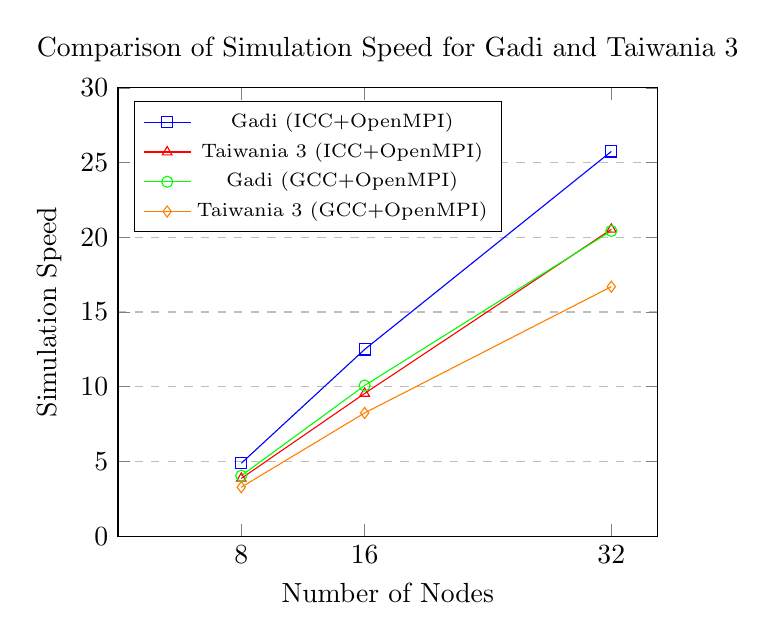
\begin{tikzpicture}
\begin{axis}[
    title={Comparison of Simulation Speed for Gadi and Taiwania 3},
    xlabel={Number of Nodes},
    ylabel={Simulation Speed},
    xmin=0, xmax=35,
    ymin=0, ymax=30,
    xtick={8, 16, 32},
    ytick={0, 5, 10, 15, 20, 25, 30},
    legend pos=north west,
    legend style={font=\scriptsize}, % 調整圖例字體大小
    ymajorgrids=true,
    grid style=dashed,
]

% ICC + OpenMPI
\addplot[
    color=blue,
    mark=square,
    ]
    coordinates {
    (8, 4.8811)(16, 12.4976)(32, 25.7474)
    };
    \addlegendentry{Gadi (ICC+OpenMPI)}

\addplot[
    color=red,
    mark=triangle,
    ]
    coordinates {
    (8, 3.8668)(16, 9.5514)(32, 20.5316)
    };
    \addlegendentry{Taiwania 3 (ICC+OpenMPI)}

% GCC + OpenMPI
\addplot[
    color=green,
    mark=o,
    ]
    coordinates {
    (8, 4.0511)(16, 10.081)(32, 20.43)
    };
    \addlegendentry{Gadi (GCC+OpenMPI)}

\addplot[
    color=orange,
    mark=diamond,
    ]
    coordinates {
    (8, 3.2786)(16, 8.2471)(32, 16.6974)
    };
    \addlegendentry{Taiwania 3 (GCC+OpenMPI)}


\end{axis}
\end{tikzpicture}
\caption{Comparison of simulation speed between Gadi and Taiwania 3 with ICC and GCC compilers and OpenMPI on testcases with different nodes.}
\label{fig:compare-compiler}
\end{figure}

\subsection{Foundational Layer Of Software Installation}
\subsubsection{C and MPI Compiler selection}
For our first approach, we've tested out different C and MPI compiler combination. The result shows ICC 2021.10.0 with OpenMPI 4.1.5 is the best suite for MPAS, which outperformed other combination when running MPAS on the 32 nodes. Additionally, performance testing was also conducted on the Taiwania 3. Fig.~\ref{fig:compare-compiler} illustrates a performance comparison between the two clusters. The network speed difference in Table.~\ref{table:hardware} is the main reason Gadi faster than Taiwania 3.

\subsubsection{OpenMPI and UCX Configuration}

we focused on optimizing both UCX (Unified Communication X)~\cite{ucx} and OpenMPI to enhance performance. UCX exposes a set of abstract communication primitives that utilize the best of available hardware resources and offloads. MPI libraries adopt UCX as their underlying communication protocol.

For UCX optimization, we deactivated all debugging flags to improve performance, and enhanced it further by enabling UD (Unreliable Datagram) and RC (Reliable Connection) support. We also integrated KNEM for shared memory-based, high-performance intra-node MPI communication.

For OpenMPI 4.1.5 optimization, we enable HCOLL~\cite{hcoll} for optimized collective communication and romio for advanced I/O handling in MPI. Additionally, we enabled Lustre support for MPI, coupled with Lustre $+$ UFS for ROMIO filesystem types~\cite{ROMIO}. We also activated sparse group support and selected the \texttt{mellanox/optimized} configuration by setting the \texttt{--with-platform} flag.

% UCX (Unified Communication X) is a communication library designed for high-performance computing, MPI libraries use underlying communication libraries to implement message-passing operations, and UCX provides a generic, efficient framework for low-level communication that can be used across various heterogeneous hardware and communication technologies. In this case, We tried to optimize the installation of UCX and MPI, In UCX, we turn off all the debugging flags since it has worse performance than other methods. We have enabled UD (Unreliable Datagram) and RC (Reliable Connection) support, and incorporated KNEM for shared memory-based high-performance intra-node MPI communication. For OpenMPI 4.1.5, we also turn off all the debugging flags. In addition, we use the hcoll and romio to support optimized communication operations, and enable the lustre support for MPI and lustre $+$ ufs for ROMIO filesystem type. Last but not least, we enable the sparse group support and use the \texttt{mellanox/optimized} option by setting \texttt{--with-platform} flag.

\subsubsection{Compile Time Flag}

We utilize the \texttt{-march} flag for CPU-specific optimizations and the \texttt{-ax} flag to create code versions for multiple architectures during compilation. Consequently, these two flags gave us some benefits on the overall integration time by 4 seconds lesser, which is almost a 10\% performance improvement. 


\subsection{Dynamic Performance Optimizations}

% \subsection{Parallel IO variables in MPAS}

% In the running file of MPAS, a file called \texttt{namelist.atmosphere} stores the parameters used in simulation. There are two variables related to Parallel IO library is \texttt{config\_pio\_num\_tasks} and \texttt{config\_pio\_strides}. The fundamental rules to tune these two variables is to keep the product of them equals to the number of MPI tasks we used, which is

% \begin{align*}
%      config\_pio\_num\_tasks \times config\_pio\_strides\\
%     = Total\;MPI\;tasks
% \end{align*}

% We tune these two parameters based on this equation, and tried with three different configurations, which are (32, 48), (48, 32), and (64, 24) for \texttt{config\_pio\_num\_tasks} and \texttt{config\_pio\_strides} respectively for 32 nodes (total 1536 MPI tasks). The result is shown in Fig.~\ref{fig:config-pio}.

% \begin{figure}[htb]
%     \centering
%     \begin{tikzpicture}
%         \begin{axis}[
%             ybar,
%             bar width=0.6cm,
%             xlabel={Configurations},
%             ylabel={Simulation Speed},
%             ymin=23.5,
%             symbolic x coords={\text{(32, 48)}, \text{(48, 32)}, \text{(64, 24)}},
%             xtick=data,
%             enlargelimits=0.5,
%         ]
%         \addplot[
%             color=orange,
%             fill=orange,
%             fill opacity=0.5
%         ] coordinates {(\text{(32, 48)}, 24.08) (\text{(48, 32)}, 24.03) (\text{(64, 24)}, 24)};
%         \end{axis}
%     \end{tikzpicture}
%     \caption{Simulation Speed with different PIO parameters in MPAS. All of them uses 32 nodes to get the best performance.}
%     \label{fig:config-pio}
% \end{figure}

% We can see that when the configurations on these two parameters matches the nodes we used and the hardware threads on each machine, MPAS performs slightly better cause they matches the number of nodes and hardware threads performing I/O operations. We've gained about 0.3\% of performance increase from here.

\subsubsection{Graph Load-Balancing}
Fig.~\ref{figure:profile-before} is our profiling result from IPM, in this figure we found that the load-balancing didn't seem well on MPAS. It can be cause by the way Metis partition the mesh and it should be able to resolve by giving Metis~\cite{metis} different setup. 

\begin{figure}[t]
    \centering
    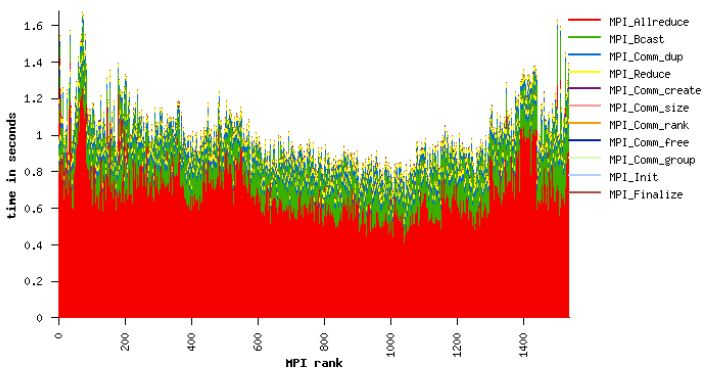
\includegraphics[width=0.5\textwidth]{profileBefore.JPG} 
    \caption{Load balancing of MPI functions according to simulation time (without I/O)}
    \label{figure:profile-before}
\end{figure}

After research, we change the load balancing tolerance in Metis. Moreover, selecting \texttt{objtype} (the mesh optimization mode) from optimization for edge cuts to optimization for communication.

\begin{table}[t]
    \centering
    \caption{Metis Configuration Comparison}
    \begin{tabular}{lll}
        \toprule
        Type & Default & Optimize  \\
        \midrule
        Objtype & Edge Cuts (cut) & Communication (vol) \\
        Edge cuts & 350158 & 347823 \\
        Communication volume & 354760 & 352425 \\
        Balance & 1.015 & 1.004 \\
        \bottomrule
    \end{tabular}
    \label{table:metis-configuration}
\end{table}

After all, the balancing issue has improved a little bit, in Fig.~\ref{figure:profile-after} the peak has dropped from 1.6 to 1.4 with a similar lower bound. We believe this issue may impact more in some longer or larger simulations.

\begin{figure}[t]
    \centering
    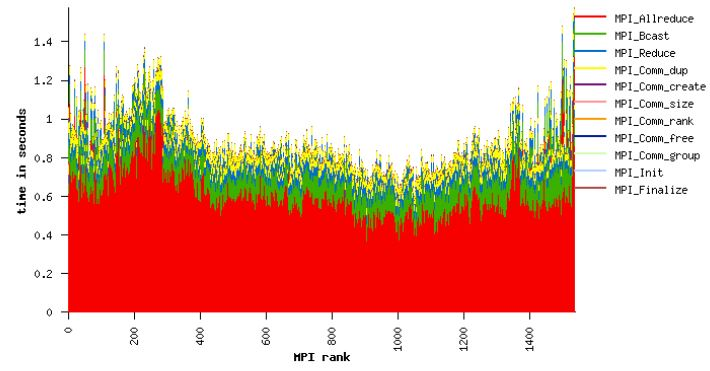
\includegraphics[width=0.5\textwidth]{profile.JPG} 
    \caption{Load balancing of MPI functions according to simulation time (without I/O) after our approach}
    \label{figure:profile-after}
\end{figure}

\subsubsection{I/O optimization}
Due to the longer integration step occurring every simulated 10 minutes, we suspect that there may have I/O operations causing delays. Thus, we've tried different I/O optimization attempts to solve this issue. A simple attempt is set some ROMIO~\cite{ROMIO} environment variables to boost up the I/O. By setting \texttt{romio\_cb\_read} or \texttt{romio\_cb\_write}, we can enable or disable to let the program select the activation of the collecting buffering. This configuration resulted in an approximated 50\% reduction in I/O time.

\subsection{Final results on Gadi and Taiwania3}
After all the approaches were done, the best results is show in Fig.~\ref{fig:speed_comparison_nodes} with a baseline.

\begin{figure}[t]
\centering
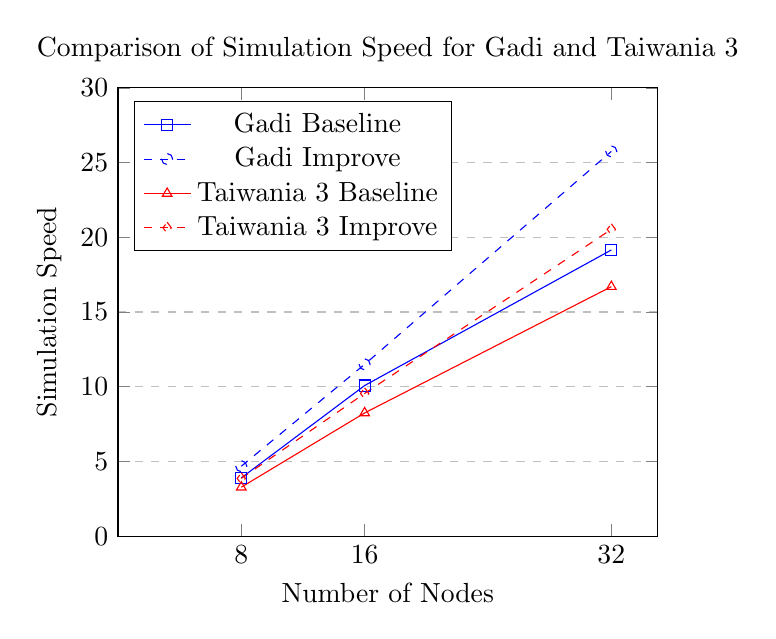
\begin{tikzpicture}
\begin{axis}[
    title={Comparison of Simulation Speed for Gadi and Taiwania 3},
    xlabel={Number of Nodes},
    ylabel={Simulation Speed},
    xmin=0, xmax=35,
    ymin=0, ymax=30,
    xtick={8, 16, 32},
    ytick={0, 5, 10, 15, 20, 25, 30},
    legend pos=north west,
    ymajorgrids=true,
    grid style=dashed,
]

% Gadi baseline
\addplot[
    color=blue,
    mark=square,
    ]
    coordinates {
    (8, 3.9037)(16, 10.081)(32, 19.1523)
    };
    \addlegendentry{Gadi Baseline}

% Gadi improve
\addplot[
    color=blue,
    mark=o,
    dashed,
    ]
    coordinates {
    (8, 4.6811)(16, 11.4976)(32, 25.7474)
    };
    \addlegendentry{Gadi Improve}

% Taiwania 3 baseline
\addplot[
    color=red,
    mark=triangle,
    ]
    coordinates {
    (8, 3.2786)(16, 8.2471)(32, 16.6974)
    };
    \addlegendentry{Taiwania 3 Baseline}

% Taiwania 3 improve
\addplot[
    color=red,
    mark=diamond,
    dashed,
    ]
    coordinates {
    (8, 3.8668)(16, 9.5514)(32, 20.5316)
    };
    \addlegendentry{Taiwania 3 Improve}

\end{axis}
\end{tikzpicture}
\caption{Simulation speed comparison between baseline and final result in Gadi and Taiwania 3.}
\label{fig:speed_comparison_nodes}
\end{figure}
